Модель достигла неплохого качества в задаче классификации: ROC-AUC=0.9, accuracy=0.82. Попробуем интерпретировать ее результаты.

\textbf{Нулевой способ это встроенный метод XGBoost}, показывающий важность признаков при предсказании. Посмотрим на первые 5 самых важных признаков. Данная величина может быть расчитана тремя способами: <<weight>>, <<gain>>, <<cover>>. Первый показывает, сколько раз признак появляется в дереве:

\begin{figure}[h]
	\centering{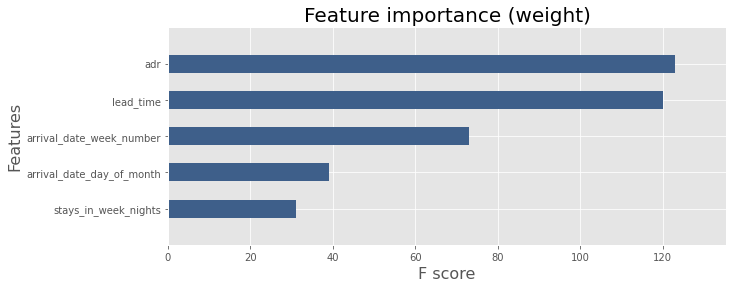
\includegraphics[width=0.85\linewidth]{pics/imp1.png}}
\end{figure}

Второй -- на сколько в среднем уменьшалась ошибка при использовании данного признака:

\begin{figure}[h]
	\centering{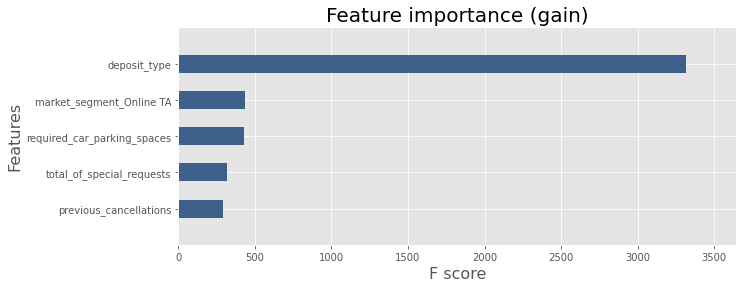
\includegraphics[width=0.85\linewidth]{pics/imp2.png}}
\end{figure}

И последний -- какое количество объектов выборки задействовало узлы с заданным признаком:

\begin{figure}[h]
	\centering{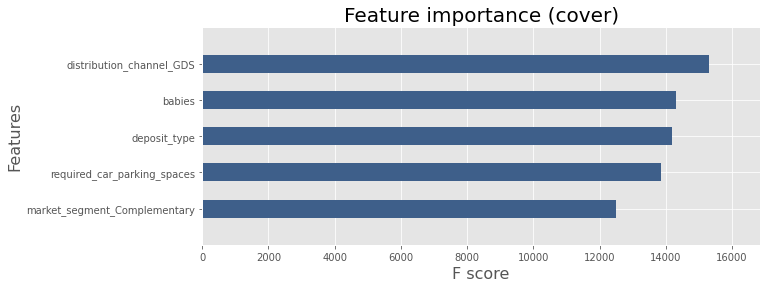
\includegraphics[width=0.85\linewidth]{pics/imp3.png}}
\end{figure}

Теперь перейдем к описанным ранее методам. \textbf{Первый -- PDP}. Возьмем признаки, которые сам XGBoost посчитал наиболее важными: первые два из weight (adr, lead\_time), первый из gain (deposit\_type) и первый из cover (distribution\_channel\_GDS) -- они с отрывом вырываются в лидеры.

И также возьмем признаки, которые XGBoost счел самыми незначительными: последний из weight (distribution\_channel\_GDS, забавно -- в тренировочной выборке всего 145 объектов, которым соответствует GDS. Судя по всему данный признак встречается 1-2 раза в узлах деревьев, но при этом он отсекает очень много объектов, из-за чего cover считает его важным), последний из gain (customer\_type\_group) и последний из cover (market\_segment\_Offline TA/TO).

Построим для них PDP.

\begin{tabular}{c|c}
	\arrayrulecolor[rgb]{0.8,0.85,1}
	\includegraphics*[width = 0.47\textwidth]{pics/mypdp1.png} & \includegraphics*[width = 0.47\textwidth]{pics/mypdp2.png}\\
	\hline
	\includegraphics*[width = 0.47\textwidth]{pics/mypdp3.png} & \includegraphics*[width = 0.47\textwidth]{pics/mypdp4.png}\\
	\hline
	\includegraphics*[width = 0.47\textwidth]{pics/mypdp5.png} & \includegraphics*[width = 0.47\textwidth]{pics/mypdp6.png}\\
\end{tabular}\\[2mm]

Первый признак является непрерывным, второй --  дискретным, третий -- порядковым, остальные -- бинарными. Для первых двух видно распределение значений признака (штриховка под графиком) и коридор, показывающий как данный признак влиял на разные объекты в выборке. Для остальных: выборка была кластеризована, и для каждого кластера из 1000 была построена усредненная по подвыборке кривая.

По графикам видно, что:
\begin{itemize}
	\item признак adr оказался важным с точки зрения PDP -- для больших значений (> 50) он вносит положительный вклад в прогноз, увеличивая вероятность отмены брони. Но видно, что для некоторых объектов в выборке он оказывал также и отрицательное влияние -- коридор задевает область отрицательных значений.
	
	Данный признак показывает, сколько в среднем гость тратит на проживание и связанные с ним расходы. Исходя из графика, можно сделать вывод, что чем больше предстоящие расходы, тем выше вероятность отмены брони -- звучит логично, клиент вероятнее отменит бронь, если для него эта поездка окажется слишком дорогой. Причем вклад данного признака стабилизируется с ростом затрат и составляет +0.2 к вероятности отмены в среднем
	
	\item Аналогичный график у lead time (время от открытия брони до приезда).
	
	Здесь ситуация также интуитивно понятна: если гость очень заранее забронировал номер, то за время до приезда его планы могут поменяться. Поэтому клиент вероятнее отменит бронь в данном случае -- +0.2-0.4 к вероятности отмены
	
	\item deposit type также оказался важным признаком: в среднем он оказывает положительное воздействие на предсказание, которое доходит вплоть до полного влияния в виде +0.9 к вероятности. Ни для одного кластера признак не оказывает отрицательное воздействие, однако возможно для отдельных объектов это неверно -- важно аккуратно интерпретировать результаты.
	
	Здесь результат несколько контринтуитивен. Если у клиента есть полный предоплаченный депозит, который не возвращается, то вероятность отмены брони стремится к единице, что нелогично -- внесенный залог должен мотивировать гостей приезжать. Далее мы видим, что для большинства кластеров при переходе к возвращаемому частичному депозиту вероятность практически не меняется и остается около единицы -- это уже более логично, однако также спорно: в случае отмены придется тратить время на бюрократию, связанную с возвратом средств. Но для части кластеров при переходе к возвращаемому депозиту вероятность отмены даже падает, что вызывает сомнения в корректности использования данного признака. Возможно, стоило выбрать другую форму для данного признака: сделать его бинарным, а не порядковым -- то есть, возможно, данная ситуация сложилась из-за неправильного представления категорий депозита.
	
	\item distribution channel GDS отрицательно влияет на предсказание, причем довольно-таки сильно: при переходе от 0 к 1 вероятность отмены брони снижается в среднем на 0.1, максимально по кластерам на 0.3
	
	Данный признак показывает то, что гость воспользовался глобальной системой бронирования, то есть вероятно самостоятельно организовал себе поездку. Снижение вероятности в данном случае не очень логично: человеку проще отменить поездку, когда он ее организовал сам. Также в таком случае выше шанс возникновения проблем в поездке (по сравнению с ораганизацией, предоставляемой туристическими агентствами), из-за чего бронь также может быть отменена
	
	\item у customer type group похожий график, однако влияние существенно ниже. Вероятность снижается на 0.04 в среднем, максимально по кластерам всего лишь на 0.1
	
	График показывает, что при организации групповой поездки ниже шанс, что она отменится. Исходно не очень понятно: если бронь на группу, то она вероятнее отменится, потому что сложно организовать путешествие на целую группу, или она вероятнее не отменится из-за, например, обязательства каждого перед другими (чтобы не ставить людей из своей группы в неудобное положение). То есть данный график приносит некоторое дополнение к нашим данным. Теперь мы знаем, что если поездка организуется для группы, то бронь скорее не будет отменена -- учитываем данное дополнение с осторожностью, учитывая неточность метода
	
	\item признак market segment offline TA/TO оказался незначительным, в среднем он вносит нулевой вклад в предсказание. Однако по кластерам видно, что разброс существенный. То есть данный признак оказывает влияние на каждый отдельный объект -- PDP в виде усредненной кривой не совсем корректный выбор для интерпретации в данном случае, так как он не учитывает разброс
\end{itemize}

Построим также графики взаимодействия признаков (PDP для двух признаков)\footnote{При построении второго типа графика (contour), который показывает линии уровня может возникнуть ошибка. Это связано с несоответствием версии библиотеки matplotlib}. Посмотрим на совместное влияние признаков, которые XGBoost по критерию weight счел важными: adr и lead time.

\begin{tabular}{c|c}
	\arrayrulecolor[rgb]{0.8,0.85,1}
	\includegraphics*[width = 0.5\textwidth]{pics/mypdp7.png} & \includegraphics*[width = 0.42\textwidth]{pics/mypdp8.png}\\
\end{tabular}\\[2mm]

Данный график показывает не влияние предикторов, а непосредственно предсказание. Действительно, взаимодействие данных признаков меняет картину (то есть предсказание не линейно зависит от них). Разброс значений наблюдается с 0.199 до 0.772, разница в 0.573. Особо выделяется пик, который сложился именно из взаимодействия -- желтый островок со значениями 0.7+

В целом мы видим, что при росте времени до приезда и затрат вероятность растет. И выделяется особый случай, когда затраты не очень большие, а время до приезда велико -- в таком случае вероятность отмены брони максимальна.
\newpage
Также интересно узнать, станет ли market segment offline TA/TO более значимым в сочетании с другим, например, с lead time.

\begin{tabular}{c|c}
	\arrayrulecolor[rgb]{0.8,0.85,1}
	\includegraphics*[width = 0.44\textwidth]{pics/mypdp9.png} & \includegraphics*[width = 0.44\textwidth]{pics/mypdp10.png}\\
\end{tabular}\\[2mm]

Рассмотрение двух признаков привело к появлению влияния market segment offline TA/TO -- при больших значениях lead time он становится более значимым, его предельный эффект при lead time $=709$ в среднем составляет $0.572-0.633=-0.06$, что по модулю больше нуля. При малых значениях lead time он перестает влиять на предсказание. Это отличается от результатов, полученных ранее.

Получили добавку к интерпретации market segment offline TA/TO -- если поездка организована туроператором, то она менее вероятно отменится, что интуитивно понятно.

С помощью PDP мы убедились в корректности восприятия моделью некоторых признаков. Для других -- в контринтуитивности результатов, а также нашли возможность для пересмотра формата признаков с целью улучшения модели. Стоит отметить, что в PDP есть очевидный недостаток -- если признак равен 0, то его влияние также равно 0, что не всегда правда. Важно обращать на это внимание при интерпретации.

\textbf{Перейдем к следующему методу -- LIME}. Рассмотрим конкретную поездку (первая из тренировочной выборки), чтобы увидеть, какие признаки оказались наиболее важными для предсказания отмены брони. Истинное значение для данного объекта: 0, то есть бронь не была отменена. 

\begin{figure}[h]
	\centering{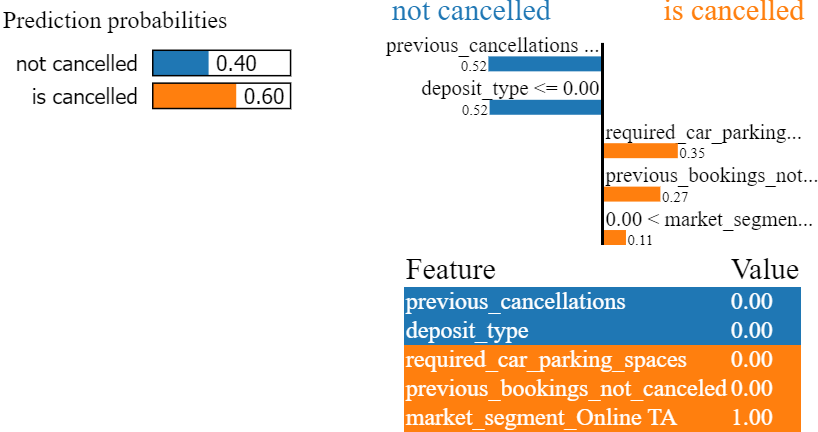
\includegraphics[width=0.7\linewidth]{pics/mylime1.png}}
\end{figure}

Модель предсказала, что бронь будет отменена, и LIME с некоторой погрешностью показывает нам, что на это повлияло. Мы видим, что отсутствие отмен ранее снизило вероятность текущей отмены, что корректно. Снова столкнулись с признаком deposit type -- отсутствие депозита также снизило вероятность отмены -- в целом не противоречит ничему, однако отсутствие депозита позволяет без каких-либо потерь отменить бронь, то есть все же скорее увеличивает вероятность отмены с точки зрения интуиции. Два данных признака сильнее всего повлияли на снижение вероятности отмены: -0.52 от каждого.

Клиент не запросил парковочное место, что увеличило вероятность отмены причем довольно-таки сильно (+0.35) -- неочевидное влияние. Отсутствие не отмененных ранее бронирований также повысило вероятность отмены, что звучит логично. Судя по всему это новый для отеля клиент. Он заказывал номер через онлайн-туроператора, и это повысило вероятность отмены на 0.11 -- интуитивно понятно, по интернету проще отменить бронь.

LIME вывел первые пять признаков, которые сильнее всего повлияли на результат. Остальные признаки довели предсказание до того, что получила модель. Она ошиблась с ответом, и мы по полученному объяснению можем понять почему. Вопросы вызывают признаки deposit type и required car parking spaces -- они оказывают неочевидное воздействие на предсказание, возможно, именно из-за них модель ошиблась. Также стоит обратить внимание на силу влияния признаков: не очень понятно, почему предикторы, снижающие вероятность отмены имеют такое большое значение. То же можно сказать и про required car parking spaces.

Таким образом, LIME позволяет выявить недостатки в понимании смысла признаков у модели. Благодаря этому мы можем предотвратить использование некорректной модели и попытаться улучшить ее.

\textbf{Посмотрим на то же самое предсказание с помощью последнего рассматриваемого метода -- SHAP}.